\begin{frame}
\frametitle{Transformed images fall on manifolds}
Rotating an image leads to points on a 1D manifold.\par
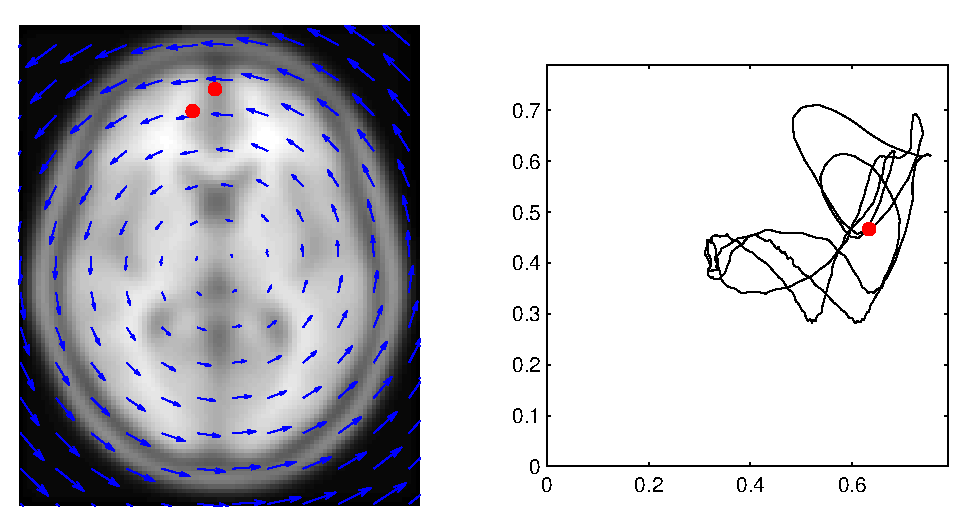
\includegraphics[width=\textwidth]{manifold_rotation}

Rigid-body motion leads to a 6-dimensional manifold (not shown).

\end{frame}

\begin{frame}
\frametitle{Local linearisation through smoothing}
\begin{columns}[c]
\column{0.7\textwidth}
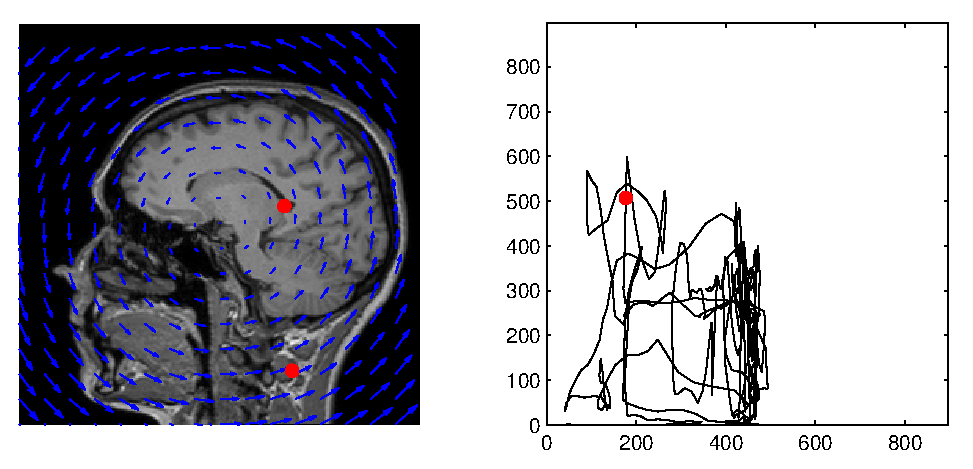
\includegraphics[width=\textwidth]{manifold_unsmoothed}\par
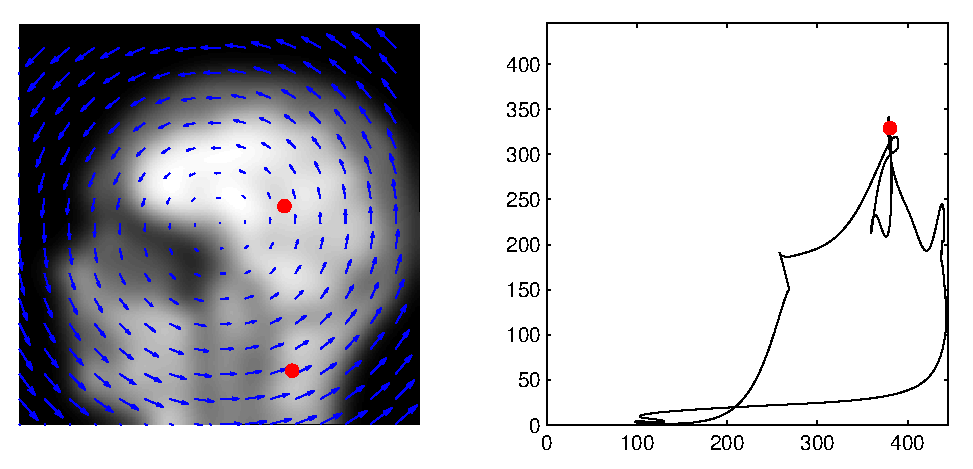
\includegraphics[width=\textwidth]{manifold_smoothed}
\column{0.3\textwidth}
Spatial smoothing can make the manifolds more linear with respect to small misregistrations.

Some information is inevitably lost.
\end{columns}
\end{frame}

\begin{frame}
\frametitle{Metrics}
Distances need to satisfy the properties of a \emph{metric}:
\begin{enumerate}
\item $d({\bf x}, {\bf y}) \ge 0$ (non-negativity)
\item $d({\bf x}, {\bf y}) = 0$ if and only if ${\bf x} = {\bf y}$ (identity of indiscernibles)
\item $d({\bf x}, {\bf y}) = d({\bf y}, {\bf x})$ (symmetry)
\item $d({\bf x}, {\bf z}) \le d({\bf x}, {\bf y}) + d({\bf y}, {\bf z})$ (triangle inequality).
\end{enumerate}

Satisfying (3) requires inverse-consistent image registration.

Satisfying (4) requires a specific class of image registration models.
\end{frame}


\begin{frame}
\frametitle{Non-Euclidean geometry}
\begin{columns}[c]
\column{0.5\textwidth}
\begin{itemize}
\item Distances are not always measured along a straight line.
\item ``\emph{Shapes are the ultimate non-linear sort of thing}''
\end{itemize}
\column{0.5\textwidth}
\includegraphics[width=\textwidth]{Globe}
\end{columns}
\end{frame}

